\documentclass[slidestop]{beamer}
\mode<presentation> {
\usetheme{Warsaw}
\setbeamercovered{transparent}}
\usepackage[czech]{babel}
\usepackage{xltxtra}

\begin{document}
\title{Obhajoba semestrální práce UAI/755}
\author{Pavel Máca}
\institute{Operační Systémy 2}
\date{\today}
%%%%%%%%%%
\begin{frame}
\titlepage
\end{frame}
%%%%%%%%%%
\begin{frame}{Osnova}
\tableofcontents
\end{frame}
%%%%%%%%%%
\section{Vyprodané speciality}
\begin{frame}
\frametitle{Vyprodané speciality}
\begin{figure}[h] % b, t, h
\begin{center}
\scalebox{0.4}{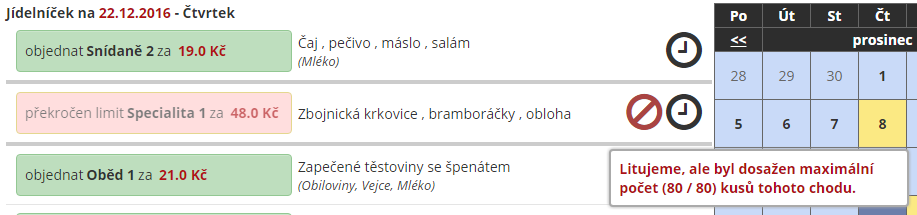
\includegraphics{nope.PNG}}
\\~\\
\scalebox{0.4}{
\includegraphics{mail.PNG}}
\end{center}
\end{figure}
\end{frame}
%%%%%%%%%%%
\section{Jak se přihlásit}
\subsection{Přihlášení k odběru}
\begin{frame}
\frametitle{Jak se přihlásit}
\begin{itemize}
\item v prohlížeči otevřít \href{https://menza-jcu.assassik.cz}{menza-jcu.assassik.cz} \pause
\begin{figure}[h] % b, t, h
\begin{center}
\scalebox{0.3}{
\includegraphics{page.PNG}}
\end{center}
\end{figure}
\item přihlásit se k odběru a počkat na notifikaci
\end{itemize}
\end{frame}
%%%%%%%%%%%%%
\subsection{Uvítací email}
\begin{frame}
\frametitle{Uvítací email}
\vfill
\begin{figure}[h] % b, t, h
\begin{center}
\scalebox{0.3}{
\includegraphics{welcome.PNG}}
\end{center}
\end{figure}
\vfill
\end{frame}
%%%%%%%%%%%%%
\section{Funkčnost}
\subsection{Technologie}
\begin{frame}
\frametitle{Použitý jazyk a systém}
\vfill
\begin{itemize}

\item Aplikce je napsána primárně v PHP za pomocí Nette\footnote{webový framework pro PHP}.

\item PHP obstarává server Nginx\footnote{http server}

\item O grafickou část se stará HTML a JS knihovna Boostrap\footnote{sada nástrojů na tvorbu webových aplikací}.

\item Emaily odesílá pomocí SMTP\footnote{protokol pro odesílání emailů} server Google

\item Celý stack běží na OS Debian

\end{itemize}
\vfill
\end{frame}
%%%%%%%%%%%%%
\subsection{Získání dat}
\begin{frame}
\frametitle{Získání dat}
\vfill
Aktuální jídelníček se získává z adresy \href{http://menza.jcu.cz/Studentska.html}{menza.jcu.cz/Studentska.html}
\\~\\
Pomocí externí knihovny je stažen HTML kód, který je dále zpracován do podoby, ve které je možné s ním pracovat v PHP skriptu.

\begin{alertblock}{PHP}
Pracuje s HTML jako s DOM objektem.
\end{alertblock}

Změny jídelníčku jsou kontrolovány pomocí cronu.
\vfill
\end{frame}
%%%%%%%%%
\subsection{Konzole}
\begin{frame}[containsverbatim]
\frametitle{Konzole}
Aplikaci lze spouštět a ovládat z příkazové řádky.
\vfill
\verb@php www/index.php <přikaz> [<argument>]@
\vfill
\begin{block}{Dostupné příkazy}
  \begin{itemize}
    \item \verb@subscribe <email>@ - Přidá email do seznamu odběratelů
    \item \verb@unsubscribe  <emai>@ - Odebere email ze seznamu odběratelů
    \item \verb@notification-send@  - Odešle notifikace, pokud existuje nový jídelníček
    \item \verb@subscription-list@ - Vypíše seznam odběratelů
  \end{itemize}
\end{block}
\vfill
\end{frame}
%%%%%%%%%
\subsection{Ukázka kódu}
\begin{frame}[containsverbatim]
\frametitle{Ukázka kódu}
\begin{figure}[h] % b, t, h
\begin{center}
\scalebox{0.55}{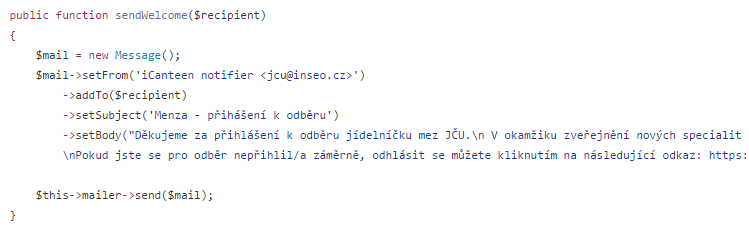
\includegraphics{code.PNG}}
\end{center}
\end{figure}
\end{frame}
%%%%%%%%%
\section{Dotazy}
\begin{frame}
\frametitle{Dotazy}
\vfill
Zdrojový kód je k dispozici na adrese:
\href{https://github.com/pavelmaca/jcu-icanteen-subscribe}{https://github.com/pavelmaca/jcu-icanteen-subscribe}

\begin{block}{Další funkce...}
  \begin{itemize}
  \item Denní notifikace na bezobjednávková jídla
  \item Automatické objednávání
  \item Další pobočky menzy
  \end{itemize}
\end{block}
\vfill
\tiny {Prezentace vytvořena pomocí \LaTeX}
\end{frame}
\end{document}